Graphs will be used in the description of semigroupoids, and provide a geometric picture which will be useful throughout this paper. The graphs we consider are sometimes called \emph{directed multigraphs}, since all edges come with a direction and we allow multiple edges between points.

\begin{definition}
A \emph{graph} is a tuple $G=(G^{(0)},G^{(1)},\so,\ra)$, where $G^{(0)}$ and $G^{(1)}$ are classes of \emph{vertices} and \emph{arrows}, respectively, and $\so,\ra\colon G^{(1)}\to G^{(0)}$ are functions, called the \emph{source} and \emph{range} maps.
\end{definition}

Alternative terminology is sometimes employed. Elements of $G^{(0)}$ are also called \emph{objects} or \emph{units}; elements of $G^{(1)}$ are called \emph{edges}; The source map is also called the \emph{domain} map, and the range map the \emph{target} or \emph{codomain} map. We may alternate between these terminologies depending on the context. If necessary, we will use subscripts to specify the graph $G$, as in writing $\so_G$ and $\ra_G$.

We usually write simply $G$ in place of $G^{(1)}$, so that an inclusion of the form $g\in G$ means that $g$ is an arrow of $G$.

Note that the source and range maps give fibred structures on $G^{(1)}$ over $G^{(0)}$. Moreover, we will generally assume that $G=\so(G)\cup\ra(G)$, in the same manner that surjective bundles are the ones of interest.

A \emph{graph morphism} $\phi\colon G\to H$ between graphs $G$ and $H$ is a pair $\phi=(\phi^{(0)},\phi^{(1)})$ of maps $\phi^{(0)}\colon G^{(0)}\to H^{(0)}$ and $\phi^{(1)}\colon G^{(1)}\to H^{(1)}$ such that $\so_H\circ\phi^{(1)}=\phi^{(0)}\circ\so_G$ and $\ra_H\circ\phi^{(1)}=\phi^{(0)}\circ\ra_G$. In other words, it is a simultaneous fibred morphism from $G$ to $H$ over their respective source and range maps. A \emph{graph isomorphism} is a graph morphism $\phi$ such that both $\phi^{(0)}$ and $\phi^{(1)}$ are bijective, and in this case $\phi^{-1}=((\phi^{(0)})^{-1},(\phi^{(1)})^{-1})$ is also a graph morphism.
\[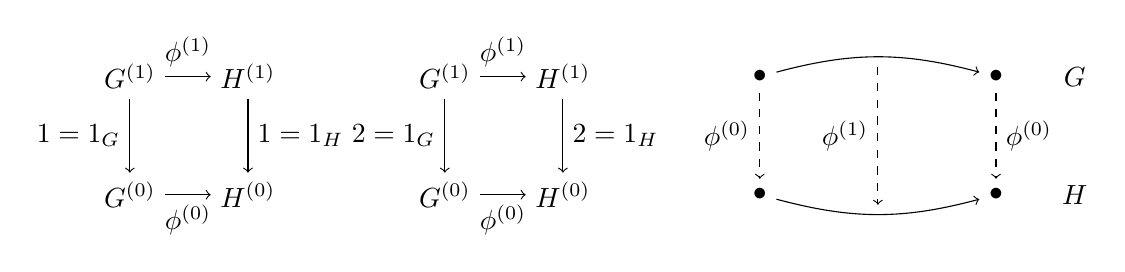
\begin{tikzpicture}
\node (G1) at (0,1) {$G^{(1)}$};
\node (G2) at ([shift={+(4,0)}]G1) {$G^{(1)}$};
\foreach \i in {1,2}
{\node (G\i2) at ([shift={+(1.5,0)}]G\i) {$H^{(1)}$};
\node (G\i3) at ([shift={+(0,-1.5)}]G\i) {$G^{(0)}$};
\node (G\i4) at ([shift={+(1.5,0)}]G\i3) {$H^{(0)}$};
\draw[->] (G\i)--(G\i2) node[above,midway] {$\phi^{(1)}$};
\draw[->] (G\i)--(G\i3) node[left,midway] {${\ifthenelse{\i=1}{\so}{\ra}}_G$};
\draw[->] (G\i3)--(G\i4) node[below,midway] {$\phi^{(0)}$};
\draw[->] (G\i2)--(G\i4) node[right,midway] {${\ifthenelse{\i=1}{\so}{\ra}}_H$};}
\node (G3) at ([shift={+(4,0)}]G2) {$\bullet$};
\node (G32) at ([shift={+(3,0)}]G3) {$\bullet$};
\node (G33) at ([shift={+(0,-1.5)}]G3) {$\bullet$};
\node (G34) at ([shift={+(0,-1.5)}]G32) {$\bullet$};
\draw[->] (G3) to[out=15,in=165] node[midway] (M1) {} (G32);
\draw[->] (G33) to[out=-15,in=195] node[midway] (M2) {} (G34);
\draw[->,dashed,thin] (M1)--(M2) node[midway,left] {$\phi^{(1)}$};
\draw[->,dashed,thin] (G3)--(G33) node[midway,left] {$\phi^{(0)}$};
\draw[->,dashed,thin] (G32)--(G34) node[midway,right] {$\phi^{(0)}$};
\node at ([shift={+(1,0)}]G32) {$G$};
\node at ([shift={+(1,0)}]G34) {$H$};
\end{tikzpicture}\]

A \emph{sink} in a graph is a vertex $v\in G^{(0)}$ such that $\so^{-1}(v)=\varnothing$. A \emph{source} in a graph is a vertex $v\in G^{(0)}$ such that $\ra^{-1}(v)=\varnothing$.
\[
    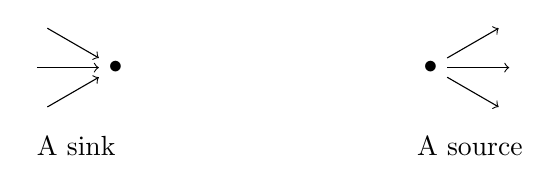
\begin{tikzpicture}
    \node (N) at (0,0) {$\bullet$};
    \node at (-0.5,-1) {A sink};
    \foreach \x in {150,180,210}
    {\draw[->] (N)+(\x:1)--(N);}
    \node (B) at (4,0) {$\bullet$};
    \node at (4.5,-1) {A source};
    \foreach \x in {0,30,330}
    {\draw[->] (B)--+(\x:1);}
    \end{tikzpicture}
\]
We will interpret the arrows of a graph as functions, and thus they will be composed from right to left, as functions are. Given $k\in\mathbb{N}_{\geq 1}$, we consider the set of \emph{$k$-paths} of a graph $G$ as
\[G^{(k)}=\left\{(g_1,\ldots,g_k)\in (G^{(1)})^ k:\so(g_i)=\ra(g_{i+1})\text{ for all }i\right\}\]
Naturally, edges of $G$ are identified with $1$-paths, so the notation $G^{(1)}$ is unambiguous in this manner. We regard $G^ {(k)}$ as a graph itself, with vertex set $G^{(0)}$ and the source and range maps given by
\[\so(g_1,\ldots,g_k)=\so(g_k)\qquad\text{and}\qquad\ra(g_1,\ldots,g_k)=\ra(g_1).\]

We also regard $G^{(0)}$ as a trivial graph with vertex set $G^{(0)}$, and the source and range maps the identity function: $\so,\ra=\id_{G^{(0)}}$.

If $G$ and $H$ are graphs over the same vertex set $G^{(0)}=H^{(0)}$, we make the fibred product $G\tensor[_{\so}]{\ast}{_{\ra}} H$ into a graph over that same vertex set, with source and range maps $\ra(g,h)=\ra(g)$ and $\so(g,h)=\so(h)$.  The construction of graphs of paths obey the ``rules of exponentiation'', where the fibred product $\tensor[_{\so}]{\ast}{_{\ra}}$ takes the role of the product: given $k,p\in\mathbb{N}_{\geq 0}$, we have natural isomorphisms
\[(G^{(k)})^{(p)}\cong G^{(pk)}\qquad\text{and}\qquad G^{(k)}\tensor[_{\so}]{\ast}{_{\ra}}G^{(p)}\cong G^{(k+p)}.\]